% Options for packages loaded elsewhere
\PassOptionsToPackage{unicode}{hyperref}
\PassOptionsToPackage{hyphens}{url}
%
\documentclass[
]{article}
\title{Rats : A normal hierarchical model}
\author{Vincent Guitteny, Freddie Joly, Tom Léchappé et Elyes Zribi}
\date{29 mars 2022}

\usepackage{amsmath,amssymb}
\usepackage{lmodern}
\usepackage{iftex}
\ifPDFTeX
  \usepackage[T1]{fontenc}
  \usepackage[utf8]{inputenc}
  \usepackage{textcomp} % provide euro and other symbols
\else % if luatex or xetex
  \usepackage{unicode-math}
  \defaultfontfeatures{Scale=MatchLowercase}
  \defaultfontfeatures[\rmfamily]{Ligatures=TeX,Scale=1}
\fi
% Use upquote if available, for straight quotes in verbatim environments
\IfFileExists{upquote.sty}{\usepackage{upquote}}{}
\IfFileExists{microtype.sty}{% use microtype if available
  \usepackage[]{microtype}
  \UseMicrotypeSet[protrusion]{basicmath} % disable protrusion for tt fonts
}{}
\makeatletter
\@ifundefined{KOMAClassName}{% if non-KOMA class
  \IfFileExists{parskip.sty}{%
    \usepackage{parskip}
  }{% else
    \setlength{\parindent}{0pt}
    \setlength{\parskip}{6pt plus 2pt minus 1pt}}
}{% if KOMA class
  \KOMAoptions{parskip=half}}
\makeatother
\usepackage{xcolor}
\IfFileExists{xurl.sty}{\usepackage{xurl}}{} % add URL line breaks if available
\IfFileExists{bookmark.sty}{\usepackage{bookmark}}{\usepackage{hyperref}}
\hypersetup{
  pdftitle={Rats : A normal hierarchical model},
  pdfauthor={Vincent Guitteny, Freddie Joly, Tom Léchappé et Elyes Zribi},
  hidelinks,
  pdfcreator={LaTeX via pandoc}}
\urlstyle{same} % disable monospaced font for URLs
\usepackage[margin=1in]{geometry}
\usepackage{graphicx}
\makeatletter
\def\maxwidth{\ifdim\Gin@nat@width>\linewidth\linewidth\else\Gin@nat@width\fi}
\def\maxheight{\ifdim\Gin@nat@height>\textheight\textheight\else\Gin@nat@height\fi}
\makeatother
% Scale images if necessary, so that they will not overflow the page
% margins by default, and it is still possible to overwrite the defaults
% using explicit options in \includegraphics[width, height, ...]{}
\setkeys{Gin}{width=\maxwidth,height=\maxheight,keepaspectratio}
% Set default figure placement to htbp
\makeatletter
\def\fps@figure{htbp}
\makeatother
\setlength{\emergencystretch}{3em} % prevent overfull lines
\providecommand{\tightlist}{%
  \setlength{\itemsep}{0pt}\setlength{\parskip}{0pt}}
\setcounter{secnumdepth}{5}
\usepackage{stmaryrd} \usepackage{float} \floatplacement{figure}{H}
\ifLuaTeX
  \usepackage{selnolig}  % disable illegal ligatures
\fi

\begin{document}
\maketitle

\newenvironment{cols}[1][]{}{}
\newenvironment{col}[1]{\begin{minipage}{#1}\ignorespaces}{%
\end{minipage}
\ifhmode\unskip\fi
\aftergroup\useignorespacesandallpars}
\def\useignorespacesandallpars#1\ignorespaces\fi{%
#1\fi\ignorespacesandallpars}
\makeatletter
\def\ignorespacesandallpars{%
  \@ifnextchar\par
    {\expandafter\ignorespacesandallpars\@gobble}%
    {}%
}
\makeatother

\renewcommand\contentsname{Table des matières}
\newpage
\tableofcontents
\newpage

\hypertarget{pruxe9sentation-du-jeu-de-donnuxe9es}{%
\section{Présentation du jeu de
données}\label{pruxe9sentation-du-jeu-de-donnuxe9es}}

Nous disposons des poids de 30 jeunes rats, mesurés chaque semaine
pendant 5 semaines. La dimension de notre jeu de données est donc de 30
par 5. Nos variables \(x_j,j=1,…,5\) correspondent aux différents âges
des rats, en jour (\(x_j = {8,15,22,29,36}\)), et nos données \(Y_{ij}\)
correspondent au poids du rat \(i\) à l'âge \(x_j\).

Un tracé des 30 courbes de croissance suggère des signes de courbure
vers le bas :

\begin{center}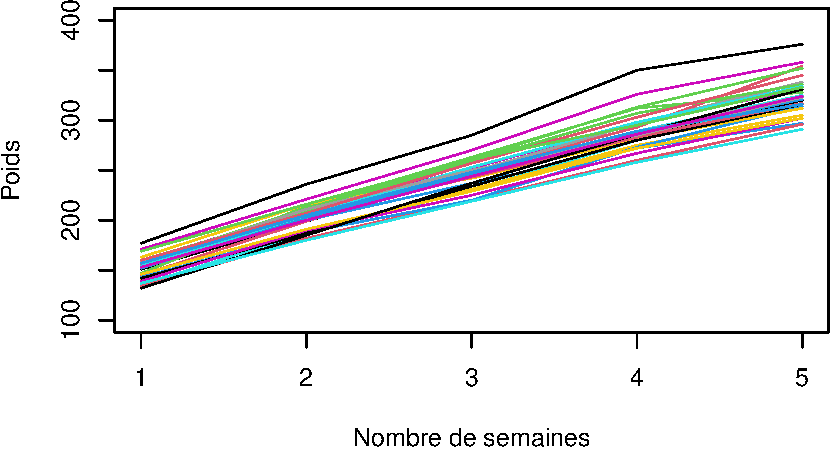
\includegraphics{Rats---A-normal-hierarchical-model_files/figure-latex/unnamed-chunk-1-1} \end{center}

\hypertarget{pruxe9sentation-du-moduxe8le}{%
\section{Présentation du modèle}\label{pruxe9sentation-du-moduxe8le}}

Le modèle est essentiellement une courbe de croissance linéaire à effets
aléatoires :

\(Y_{ij} \sim \mathcal N(\alpha_i + \beta_i(x_j - \bar x), \sigma_c ^2)\)
où \(\bar x = 22\) et \(\sigma_c ^2 \sim InvGamma(a_c,b_c)\)
(\(\sigma_c ^2\) a une loi a priori non informative)

\(\alpha_i \sim \mathcal N(\alpha_c,\sigma_{\alpha}^2)\)

\(\beta_i \sim \mathcal N(\beta_c,\sigma_{\beta}^2)\).

On note l'absence de paramètre représentant la corrélation entre
\(\alpha_i\) et \(\beta_i\). Pour l'instant, nous standardisons les
\(x_j\) autour de leur moyenne pour réduire la dépendance entre
\(\alpha_i\) et \(\beta_i\) dans leur vraisemblance : en fait, pour les
données entièrement équilibrées (centrées et réduites), une indépendance
complète est atteinte (notons qu'en général, l'indépendance a priori
n'oblige pas les distributions a posteriori à être indépendantes).

Les paramètres
\(\alpha_c, \sigma_{\alpha}^2, \beta_c, \sigma_{\beta}^2\) ont des loi a
priori « non informatives » et indépendantes :

\(\alpha_c \sim\mathcal N(0,\sigma_a^2)\)

\(\sigma_{\alpha}^2 \sim InvGamma(a_{\alpha},b_{\alpha})\)

\(\beta_c \sim \mathcal N(0,\sigma_b^2)\)

\(\sigma_{\beta}^2 \sim InvGamma(a_{\beta},b_{\beta})\).

\hypertarget{calculs-des-lois-conditionnelles-pleines}{%
\section{Calculs des lois conditionnelles
pleines}\label{calculs-des-lois-conditionnelles-pleines}}

Afin de mettre en oeuvre un algorithme MCMC (Monte Carlo Markov Chain),
à l'aide de la fonction \texttt{mcmc} du package \texttt{coda}, sur une
chaîne de Markov obtenue par un échantilloneur de Gibbs, nous avons eu
la nécessité de calculer les lois conditionnelles pleines (loi
conditionnellement aux autres paramètres) des paramètres \(\alpha_c\),
\(\beta_c\), \(\sigma_{\alpha}^2\), \(\sigma_{\beta}^2\),
\(\sigma_c ^2\), \(\alpha_i\) et \(\beta_i\) (et de voir si celles-ci
étaient identifiables). Les paramètres \(\alpha_c\), \(\beta_c\),
\(\alpha_i\) et \(\beta_i\) ont des lois a priori gaussiennes et les
paramètres \(\sigma_{\alpha}^2\), \(\sigma_{\beta}^2\) et
\(\sigma_c ^2\) ont des lois a priori inverses gamma. Nous donnons
ci-dessous un exemple de calcul pour une loi gaussienne et un exemple
pour une loi inverse gamma (le reste des démonstrations se trouve en
annexe).

\hypertarget{exemple-de-calcul-avec-des-lois-gaussiennes}{%
\subsection{Exemple de calcul avec des lois
gaussiennes}\label{exemple-de-calcul-avec-des-lois-gaussiennes}}

Dans cet exemple, on cherche à calculer la loi conditionnelle pleine du
paramètre \(\alpha_c\). Pour cela, nous avons besoin de la loi a priori
de \(\alpha_{c} \sim \mathcal{N}(O,\,\sigma_{a}^{2})\) et de la loi de
\(\alpha_{i} \sim \mathcal{N}(\alpha_{c},\,\sigma_{\alpha}^{2})\).

\begin{align*}
\Pi(\alpha_{c}|...) &\propto \Pi(\alpha_{c}) \prod_{i=1}^{n_{i}} \Pi(\alpha_{i}|\alpha_{c},\sigma_{\alpha}^{2} ) \\
        &\propto \exp\left(\frac{-\alpha_{c}^{2}}{2\sigma_{a}^{2}}\right)\prod_{i=1}^{n_{i}} \exp\left(\frac{-(\alpha_{i}-\alpha_{c})^{2}}{2\sigma_{\alpha}^{2}}\right) \\
        &\propto \exp\left(\frac{-\alpha_{c}^{2}}{2\sigma_{a}^{2}}\right)\prod_{i=1}^{n_{i}} \exp\left(\frac{-(\alpha_{c}^{2}-2\alpha_{i}\alpha_{c})}{2\sigma_{\alpha}^{2}}\right) \\
        &\propto \exp\left(\frac{-\alpha_{c}^{2}}{2\sigma_{a}^{2}}\right) \exp\left(\frac{-n_i\alpha_{c}^{2}+2\alpha_{c}\sum\limits_{i=1}^{n_{i}} \alpha_{i}}{2\sigma_{\alpha}^{2}}\right)\\
        &\propto \exp\left(\frac{-\alpha_{c}^{2}(\sigma_{\alpha}^{2}+n_i\sigma_{a}^{2}) +2\alpha_{c}\sigma_{a}^{2}\sum\limits_{i=1}^{n_{i}} \alpha_{i}}{2\sigma_{a}^{2}\sigma_{\alpha}^{2}}\right)\\
        &\sim \mathcal{N}\left(\frac{\sigma_{a}^{2}\sum\limits_{i=1}^{n_{i}} \alpha_{i}}{\sigma_{\alpha}^{2}+n_{i}\sigma_{a}^{2}},\frac{\sigma_{a}^{2}\sigma_{\alpha}^{2}}{\sigma_{\alpha}^{2}+n_{i}\sigma_{a}^{2}}\right)
\end{align*}

\hypertarget{exemple-de-calcul-avec-des-lois-inverses-gamma}{%
\subsection{Exemple de calcul avec des lois inverses
gamma}\label{exemple-de-calcul-avec-des-lois-inverses-gamma}}

Ici nous calculons la loi conditionnelle pleine du paramètre
\(\sigma_{\alpha}^2\). Pour cela, nous avons besoin de la loi a priori
de \(\sigma_{\alpha}^{2} \sim InvGamma(a_{\alpha},b_{\alpha})\) et de la
loi de
\(\alpha_{i} \sim \mathcal{N}(\alpha_{c},\,\sigma_{\alpha}^{2})\).

\begin{align*}
\Pi(\sigma_{\alpha}^{2}|...) &\propto \Pi(\sigma_{\alpha}^{2}) \prod_{i=1}^{n_{i}}\Pi(\alpha_{i}|\alpha_{c},\sigma_{\alpha}^{2}) \\
&\propto \exp^{\frac{-b_{\alpha}}{\sigma_{\alpha}^{2}}}(\sigma_{\alpha}^{2})^{-a_{\alpha}-1}\prod_{i=1}^{n_{i}} \exp\left(\frac{-(\alpha_{i}-\alpha_{c})^{2}}{2\sigma_{\alpha}^{2}}\right)(\sigma_{\alpha}^{2})^{-\frac{1}{2}}\\
&\propto (\sigma_{\alpha}^{2})^{-a_{\alpha}-1-\frac{n_{i}}{2}}\exp\left(\frac{-2b_{\alpha}-\sum\limits_{i=1}^{n_{i}}(\alpha_{i}-\alpha_{c})^{2}}{2\sigma_{\alpha}^{2}}\right)\\
&\sim InvGamma(\frac{n_{i}}{2}+a_{\alpha},\frac{2b_{\alpha}+\sum\limits_{i=1}^{n_{i}}(\alpha_{i}-\alpha_{c})^{2}}{2})
\end{align*}

\hypertarget{impluxe9mentation-et-ruxe9sultats}{%
\section{Implémentation et
résultats}\label{impluxe9mentation-et-ruxe9sultats}}

Maintenant que nous avons obtenues et identifiées toutes nos lois
conditionnelles pleines de nos paramètres, nous avons pu implémenter un
échantilloneur de Gibbs et utiliser un algorithme MCMC sur la chaîne de
Markov obtenue par cet échantilloneur.

\newpage

\hypertarget{annexes}{%
\section{Annexes}\label{annexes}}

\hypertarget{loi-conditionnelle-pleine-du-paramuxe8tre-beta_c}{%
\subsection{\texorpdfstring{Loi conditionnelle pleine du paramètre
\(\beta_c\)}{Loi conditionnelle pleine du paramètre \textbackslash beta\_c}}\label{loi-conditionnelle-pleine-du-paramuxe8tre-beta_c}}

\begin{align*}
\Pi(\beta_{c}|...) &\propto \Pi(\beta_{c}) \prod_{i=1}^{n_{i}} \Pi(\beta_{i}|\beta_{c},\sigma_{\beta}^{2} ) \\
        &\propto \exp\left(\frac{-\beta_{c}^{2}}{2\sigma_{b}^{2}}\right)\prod_{i=1}^{n_{i}} \exp\left(\frac{-(\beta_{i}-\beta_{c})^{2}}{2\sigma_{\beta}^{2}}\right) \\
        &\propto \exp\left(\frac{-\beta_{c}^{2}}{2\sigma_{b}^{2}}\right)\prod_{i=1}^{n_{i}} \exp\left(\frac{-(\beta_{c}^{2}-2\beta_{i}\beta_{c})}{2\sigma_{\beta}^{2}}\right) \\
        &\propto \exp\left(\frac{-\beta_{c}^{2}}{2\sigma_{b}^{2}}\right) \exp\left(\frac{-n_i\beta_{c}^{2}+2\beta_{c}\sum\limits_{i=1}^{n_{i}} \beta_{i}}{2\sigma_{\beta}^{2}}\right)\\
        &\propto \exp\left(\frac{-\beta_{c}^{2}(\sigma_{\beta}^{2}+n_i\sigma_{b}^{2}) +2\beta_{c}\sigma_{b}^{2}\sum\limits_{i=1}^{n_{i}} \beta_{i}}{2\sigma_{b}^{2}\sigma_{\beta}^{2}}\right)\\
        &\sim \mathcal{N}\left(\frac{\sigma_{b}^{2}\sum\limits_{i=1}^{n_{i}} \beta_{i}}{\sigma_{\beta}^{2}+n_{i}\sigma_{b}^{2}},\frac{\sigma_{b}^{2}\sigma_{\beta}^{2}}{\sigma_{\beta}^{2}+n_{i}\sigma_{b}^{2}}\right)
\end{align*}

\hypertarget{loi-conditionnelle-pleine-du-paramuxe8tre-alpha_i}{%
\subsection{\texorpdfstring{Loi conditionnelle pleine du paramètre
\(\alpha_i\)}{Loi conditionnelle pleine du paramètre \textbackslash alpha\_i}}\label{loi-conditionnelle-pleine-du-paramuxe8tre-alpha_i}}

\begin{align*}
\Pi(\alpha_{i}|...) &\propto \Pi(\alpha_{i}|\alpha_{c},\sigma_{\alpha}^{2} ) \prod_{j=1}^{n_{j}} \Pi(Y_{ij}|\alpha_{i},\beta_{i},\sigma_{c}^{2} ) \\
        &\propto \exp\left(\frac{-(\alpha_{i}-\alpha_{c})^{2}}{2\sigma_{\alpha}^{2}}\right) \prod_{j=1}^{n_{j}} \exp\left(\frac{-(y_{ij}-\alpha_{i}-\beta_i(x_{j}-\bar{x}))^{2}}{2\sigma_{c}^{2}}\right) 
\end{align*}

En posant \(\mu_{ij} = y_{ij} - \beta_i(x_{j}-\bar{x})\), on a

\begin{align*}
\Pi(\alpha_{i}|...)&\propto \exp\left(\frac{-\alpha_i^2+2\alpha_i\alpha_c}{2\sigma_{\alpha}^{2}}\right) \prod_{j=1}^{n_{j}} \exp\left(\frac{-(\alpha_{i}-\mu_{ij})^{2}}{2\sigma_{c}^{2}}\right)  \\
        &\propto \exp\left(\frac{-\alpha_i^2+2\alpha_i\alpha_c}{2\sigma_{\alpha}^{2}}\right) \prod_{j=1}^{n_{j}} \exp\left(\frac{-\alpha_i^2+2\alpha_i\mu_{ij}}{2\sigma_{c}^{2}}\right)  \\
        &\propto \exp\left(\frac{-\alpha_i^2(\sigma_c^2+n_j\sigma_{\alpha}^2) +2\alpha_i(\alpha_c\sigma_c^2+\sigma_{\alpha}^2\sum\limits_{j=1}^{n_j} \mu_{ij})}{2\sigma_{\alpha}^{2}\sigma_c^2}\right)\\
        &\sim \mathcal{N}\left(\frac{\alpha_c\sigma_c^2+\sigma_{\alpha}^2\sum\limits_{j=1}^{n_j} \mu_{ij}}{\sigma_c^2+n_j\sigma_{\alpha}^2},\frac{\sigma_{\alpha}^{2}\sigma_c^2}{\sigma_c^2+n_j\sigma_{\alpha}^2}\right)
\end{align*}

\hypertarget{loi-conditionnelle-pleine-du-paramuxe8tre-beta_i}{%
\subsection{\texorpdfstring{Loi conditionnelle pleine du paramètre
\(\beta_i\)}{Loi conditionnelle pleine du paramètre \textbackslash beta\_i}}\label{loi-conditionnelle-pleine-du-paramuxe8tre-beta_i}}

\begin{align*}
\Pi(\beta_{i}|...) &\propto \Pi(\beta_{i}|\beta_{c},\sigma_{\beta}^{2} ) \prod_{j=1}^{n_{j}} \Pi(Y_{ij}|\alpha_{i},\beta_{i},\sigma_{c}^{2} ) \\
        &\propto \exp\left(\frac{-(\beta_{i}-\beta_{c})^{2}}{2\sigma_{\beta}^{2}}\right) \prod_{j=1}^{n_{j}} \exp\left(\frac{-(y_{ij}-\alpha_{i}-\beta_i(x_{j}-\bar{x}))^{2}}{2\sigma_{c}^{2}}\right) 
\end{align*}

En posant \(\mu_{ij} = y_{ij} - \alpha_i\), on a

\begin{align*}
\Pi(\beta_{i}|...)&\propto \exp\left(\frac{-\beta_i^2+2\beta_i\beta_c}{2\sigma_{\beta}^{2}}\right) \prod_{j=1}^{n_{j}} \exp\left(\frac{-(\beta_{i}(x_{j}-\bar{x})-\mu_{ij})^{2}}{2\sigma_{c}^{2}}\right)  \\
        &\propto \exp\left(\frac{-\beta_i^2+2\beta_i\beta_c}{2\sigma_{\beta}^{2}}\right) \prod_{j=1}^{n_{j}} \exp\left(\frac{-\beta_i^2(x_{j}-\bar{x})^2+2\beta_i(x_{j}-\bar{x})\mu_{ij}}{2\sigma_{c}^{2}}\right)  \\
        &\propto \exp\left(\frac{-\beta_i^2(\sigma_c^2+\sigma_{\beta}^2\sum\limits_{j=1}^{n_j}(x_{j}-\bar{x})^2) +2\beta_i(\beta_c\sigma_c^2+\sigma_{\beta}^2\sum\limits_{j=1}^{n_j} (x_{j}-\bar{x})\mu_{ij})}{2\sigma_{\beta}^{2}\sigma_c^2}\right)\\
        &\sim \mathcal{N}\left(\frac{\beta_c\sigma_c^2+\sigma_{\beta}^2\sum\limits_{j=1}^{n_j} (x_{j}-\bar{x})\mu_{ij}}{\sigma_c^2+\sigma_{\beta}^2\sum\limits_{j=1}^{n_j}(x_{ij}-\bar{x})^2},\frac{\sigma_{\beta}^{2}\sigma_c^2}{\sigma_c^2+\sigma_{\beta}^2\sum\limits_{j=1}^{n_j}(x_{j}-\bar{x})^2}\right)
\end{align*}

\hypertarget{loi-conditionnelle-pleine-du-paramuxe8tre-sigma_beta2}{%
\subsection{\texorpdfstring{Loi conditionnelle pleine du paramètre
\(\sigma_{\beta}^2\)}{Loi conditionnelle pleine du paramètre \textbackslash sigma\_\{\textbackslash beta\}\^{}2}}\label{loi-conditionnelle-pleine-du-paramuxe8tre-sigma_beta2}}

\begin{align*}
\Pi(\sigma_{\beta}^{2}|...) &\propto \Pi(\sigma_{\beta}^{2}) \prod_{i=1}^{n_{i}}\Pi(\beta_{i}|\beta_{c},\sigma_{\beta}^{2}) \\
&\propto \exp^{\frac{-b_{\beta}}{\sigma_{\beta}^{2}}}(\sigma_{\beta}^{2})^{-a_{\beta}-1}\prod_{i=1}^{n_{i}} \exp\left(\frac{-(\beta_{i}-\beta_{c})^{2}}{2\sigma_{\beta}^{2}}\right)(\sigma_{\beta}^{2})^{-\frac{1}{2}}\\
&\propto (\sigma_{\beta}^{2})^{-a_{\beta}-1-\frac{n_{i}}{2}}\exp\left(\frac{-2b_{\beta}-\sum\limits_{i=1}^{n_{i}}(\beta_{i}-\beta_{c})^{2}}{2\sigma_{\beta}^{2}}\right)\\
&\sim InvGamma(\frac{n_{i}}{2}+a_{\beta},\frac{2b_{\beta}+\sum\limits_{i=1}^{n_{i}}(\beta_{i}-\beta_{c})^{2}}{2})
\end{align*}

\hypertarget{loi-conditionnelle-pleine-du-paramuxe8tre-sigma_c2}{%
\subsection{\texorpdfstring{Loi conditionnelle pleine du paramètre
\(\sigma_{c}^2\)}{Loi conditionnelle pleine du paramètre \textbackslash sigma\_\{c\}\^{}2}}\label{loi-conditionnelle-pleine-du-paramuxe8tre-sigma_c2}}

\begin{align*}
\Pi(\sigma_c^2|...) &\propto \Pi(\sigma_c^2) \prod_{i=1}^{n_i}\prod_{j=1}^{n_j}\Pi(Y_{ij}|\alpha_{i},\beta_{i} \sigma_c^2)
\end{align*}

En posant \(\mu_{ij} = \alpha_i + \beta_i(x_j-\bar{x})\), on a

\begin{align*}
\Pi(\sigma_c^2|...) &\propto \exp^{\frac{-b_c}{\sigma_c^2}}(\sigma_c^2)^{-a_c-1}\prod_{i=1}^{n_i}\prod_{j=1}^{n_j} \exp\left(\frac{-(y_{ij}-\mu_{ij})^{2}}{2\sigma_c^2}\right)(\sigma_c^2)^{-\frac{1}{2}}\\
&\propto (\sigma_c^2)^{-a_c-1-\frac{n}{2}}\exp\left(\frac{-2b_c-\sum\limits_{i=1}^{n_i}\sum\limits_{j=1}^{n_j}(y_{ij}-\mu_{ij})^{2}}{2\sigma_c^2}\right)\\
&\sim InvGamma(\frac{n}{2}+a_c,\frac{2b_c+\sum\limits_{i=1}^{n_i}\sum\limits_{j=1}^{n_j}(y_{ij}-\mu_{ij})^{2}}{2})
\end{align*}

\end{document}
